\documentclass[a4paper]{book}
\usepackage{a4wide}
\usepackage{makeidx}
\usepackage{fancyhdr}
\usepackage{graphicx}
\usepackage{multicol}
\usepackage{float}
\usepackage{textcomp}
\usepackage{alltt}
\usepackage{doxygen}
\usepackage[varg]{pxfonts}
\usepackage[linktocpage,
            pdfpagelabels,
            pagebackref=true,
            colorlinks=true,
            linkcolor=blue
           ]{hyperref}
\makeindex
\setcounter{tocdepth}{1}
\renewcommand{\footrulewidth}{0.4pt}
\makeatletter
\renewcommand{\l@section}{\@dottedtocline{1}{1.5em}{3.4em}}
\makeatother
\begin{document}
\begin{titlepage}
\vspace*{3cm}
\begin{center}
    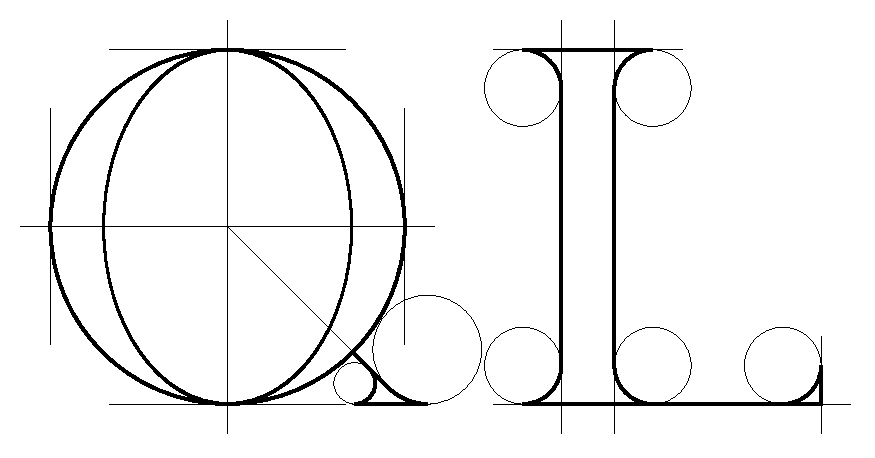
\includegraphics[width=10cm]{QL}\\
    {\Huge \bf QuantLib}\\
    \vspace*{0.5cm}
    {\LARGE \bf An open source library for quantitative finance}\\
    \vspace*{0.5cm}
    {\Large Version $projectnumber}\\
    \vspace*{5cm}
    {\large Generated by Doxygen $doxygenversion}\\
    \vspace*{0.5cm}
    {\small $date}\\
\end{center}
\end{titlepage}
\clearemptydoublepage
\pagenumbering{roman}
\tableofcontents
\clearemptydoublepage
\pagenumbering{arabic}

% Introduction

\hypertarget{qlintro}{}\chapter{Getting started}\label{qlintro}
\input{index}
\include{overview}
\include{where}
\include{install}
\include{config}
\include{usage}
\include{faq}
\include{history}
\include{resources}
\include{group}
\include{license}


% Reference manual - generated by Doxygen
